\documentclass[journal,onecolumn]{IEEEtran}

\title{Applied Spatial and Temporal Data Analysis}
\author{Vijay K. Shah}

\usepackage{amsmath}
\usepackage{mathtools}
\usepackage{graphicx}
\usepackage{enumitem}
\usepackage{epsfig}
\usepackage{color}
\usepackage{algorithm}
\usepackage[noend]{algpseudocode}
\usepackage{subfigure}
\usepackage[justification=centering]{caption}

\begin{document}
\maketitle

\section{\textbf{Data Retrieval}}

\textit{Q 1. Find 100 CNN news articles online (try to find them in different categories, e.g., sports and
finance). You need to find the new article by yourself. Pls ignore picture or other non-text data
in the new article.} \\

In this section, I first describe how 100 CNN News links were retrieved followed by the discussion on data retrieval from each link. \textbf{Note:} I actually crawled 200 CNN News articles for this assignment.

\subsection{\underline{100 CNN News Link Retrieval}:}

\begin{itemize}[label={}]
\item \textbf{Step 1:} I downloaded the urls for all the articles in the webpage - http://www.cnn.com/US/archive/

\item \textbf{Step 2:} I stored them in a text file \textbf{links.txt} in home folder \textbf{helloProject}. 

\end{itemize}
Step 1 and 2 are handled by script file \textbf{cnn\_spider.py} stored in folder \textbf{helloProject/helloProject/Spiders/}


\subsection{\underline{Data (Articles) Retrieval from all links}:}

I created a script \textbf{pages\_spider.py} to navigate through all urls (stored in links.txt) and download the content body using Scrappy request. Here, I used Scrapy selector.xpath('//p/text()') ,  selector.xpath('//h/text()') and  selector.xpath('//span/text()') so that only useful texts are downloaded instead of entire html file. After that, I only consider alphabetical words with atleast 3 alphabets using a regrex [a-zA-Z]$\{3,\}$ \\


\textbf{Note: } The script \textbf{pages\_spider.py} can be found in folder "helloProject/helloProject/Spiders"
Each downloaded article is stored as article- \textbf{article\_\%Article-headerName\%.txt} in folder \textbf{Articles/}


\begin{figure}[h]
\begin{center}
 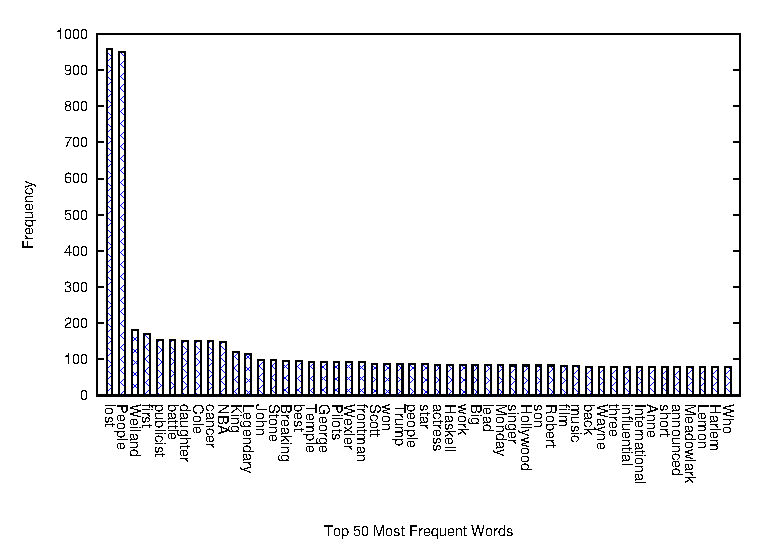
\includegraphics[width = 6.5in, height = 3.5 in] {Plots/wordFreq_allArticles.eps}
 \caption {Frequency vs Top K features (most frequent) }
 \end{center}
\end{figure}



\section{\textbf{Feature Selection}}
\textit{Q 2. Convert them to data matrix (each row is an article and each column is a unique term).}\\

In this section, I present the details of forming a data matrix where each row is an article and each column is a unique word.

\subsection{\underline{Creation of data matrix}}

\begin{itemize}[label={}]

\item \textbf{Step 1: }  I filtered out insignificant words from the data retrieved from each article as discussed in Homework 1.

\item \textbf{Step 2:} I sorted out the list of words in decreasing order of its frequency. (only until I get first  top K frequent unique words).

\item \textbf{Step 3:} I created a data matrix of size (Number of Articles) X (Top K Most Frequent Words). Each cell contains the frequency of each unique word (Column) for following article (Row).

\end{itemize} 

\subsection{\underline{Addition of \textit{Category} Column to the data matrix}}

I have added a new column called \textit{Category}, which represents the category of the article (row). The category list is as follows:
\begin{itemize}
\item \textbf{entertainment}
\item \textbf{us}
\item \textbf{health}
\item \textbf{politics}
\item \textbf{opinions}
\end{itemize}

\iffalse
\begin{table}
\scriptsize
\centering
\caption {List of Categories}  \label{Category}
\begin{tabular}{|c|} 
\hline % inserts single horizontal line
entertainment \\
\hline
 us \\
 \hline
 health \\
 \hline
 politics \\
 \hline
 opinions\\
\hline
\end{tabular}
\end{table}
\fi


\section{Classifier}
\textit{Q 3. Run kNN and Decision Tree with 5-folder cross validation. (label each cnn new article with the
category)}

I used \textbf{sklearn} to run both kNN and Decision Tree with 5-folder cross validation.
The schematic pseudocode for Decision Tree Classifier is given in Algorithm \ref{tree}.


\begin{algorithm}
\caption{DecisionTreeClassifier}\label{tree}
\begin{algorithmic}[1]

\Procedure{decisionTreeClassifier()}{} 

\State df = pd.read\_csv("dataMatrix.csv") \textit{Comment: Read the data matrix csv file}\\

\State \textit{Comment: Convert non-numerical label "Category" to numerical label}
\State label\_encoder = preprocessing.LabelEncoder()
\State encoded\_category = label\_encoder.fit\_transform(df["Category"]) \\

\State \textit{Comment: call Decision Tree classifier}
\State tree\_model = tree.DecisionTreeClassifier() \label{classifierStep} \\

\State \textit{Comment: cross validation with 5 folds}
\State cv = KFold(n=len(df), n\_folds=5)     \textit{Number of folds is 5}   \\  
       
\For  {train\_index, valid\_index in cv}
\State train = df.loc[train\_index]  \textit{Comment: Extract train data with cv indices}
\State valid = df.loc[valid\_index] \textit{Comment: Extract valid data with cv indices} \\

\State \textit{Comment: training dataset (4 folds out of 5 folds)}
\State ytrain = label\_encoder.fit\_transform(train["Category"])
\State Xtrain = train[list(train.columns[1:50])] \\

\State \textit{ Comment: test dataset (1 fold out of 5 folds)}
\State ytest = label\_encoder.fit\_transform(valid["Category"])
\State Xtest = valid[list(valid.columns[1:50])] \\

\State \textit{Comment: Predict the test dataset with the decision tree classifier}
\State y\_pred = tree\_model.predict(Xtest) \\

\State \textit{Comment: Accuracy and F-Score}
\State ac\_score = accuracy\_score(ytest, y\_pred)
\State fscore = f1\_score(ytest, y\_pred, average = "weighted")

\EndFor

\EndProcedure
\end{algorithmic}
\end{algorithm}

\textbf{Note:} For kNN classifier, only one change has to be made, which is as follows:
In Step \ref{classifierStep}, instead of DecisionTreeClassifier, KNeighborsClassifier has to be called.

	\textbf{knnClassifier = neighbors.KNeighborsClassifier(n\_neighbors=5)}
	
\section{\textbf{ Analysis}}
\textit{Q 4. Evaluate classification results with accuracy, F-measure} \\
In this section, I first define the metrics (i) Accuracy and (ii) F-measure following the evaluation of classification results.

\subsection{\underline{Accuracy}}
Accuracy is defined as the number of correct predictions made divided by the total number of predictions made, multiplied by 100.
Let $N_c$ be the number of correct predictions made and $N_t$ be the total number of predictions made, then, the accuracy is calculated as
\begin{equation}
Accuracy = \frac{N_c}{N_t} \times 100
\end{equation}

\subsection{\underline{F-measure}}


\begin{figure}[h]
\begin{center}
 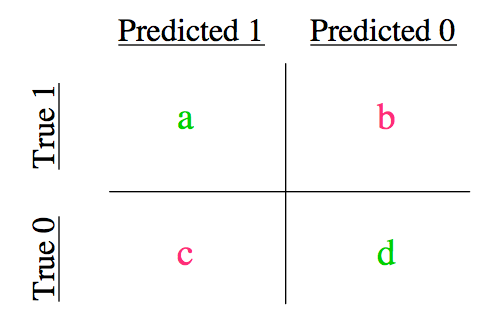
\includegraphics[scale=0.4] {Plots/f1Score.png}
 \caption {Precision/Recall} \label{precision}
 \end{center}
\end{figure}


To understand F-measure, it is important to define two parameters: (i) Precision and (ii) Recall.
\subsubsection{\textbf{Precision}}
Precision is defined as the number of True Positives divided by the number of True Positives and False Positives. In other words, it is the number of positive predictions divided by number of positive class values predicted. 

Taking Fig. \ref{precision} as a reference, the precision can be calculated as

\begin{equation}
Precision = \frac{a}{a+c}
\end{equation}


\subsubsection{\textbf{Recall}}
Recall is defined as the number of True Positives divided by number of True Positives and number of False Negatives. In other words, it is the number of positive predictions divided by the number of positive class values in the test data.

Taking Fig. \ref{precision} as a reference, the recall can be calculated as

\begin{equation}
Recall = \frac{a}{a+b}
\end{equation}

F-Score is the harmonic mean of precision and recall, calculated as follows:
\begin{equation}
F-Score = 2 \times \frac{precision \times recall }{precision + recall}
\end{equation}


\subsection{\underline{Evaluation of Decision Tree Classifier }}
In this section, we evaluate the performance of decision tree classifier in terms of Accuracy and F-Score.
\begin{figure}[h]
\begin{center}
\label{thr}
\subfigure[\label{accuracy1}]{
\epsfig{figure=Output/newTree/accuracy_unshuffled.eps,width=2.5in,keepaspectratio}}
\subfigure[\label{accuracy2}]{
\epsfig{figure=Output/newTree/accuracy.eps,width=2.5in,keepaspectratio}}
\caption{ Decision Tree Classifier: Accuracy vs (a. Unshuffled Data Matrix  b. Shuffled Data Matrix) }

\end{center}
\end{figure}

\begin{figure}[h]
\begin{center}
\label{thr}
\subfigure[\label{fscore1}]{
\epsfig{figure=Output/newTree/fScore_unshuffled.eps,width=2.50in,keepaspectratio}}
\subfigure[\label{fscore2}]{
\epsfig{figure=Output/newTree/fScore.eps,width=2.50in,keepaspectratio}}
\caption{ Decision Tree Classifier: F-Score vs (a. Unshuffled Data Matrix  b. Shuffled Data Matrix) }

\end{center}
\end{figure}

\iffalse
\begin{figure}[h]
\begin{center}
\label{thr}
\subfigure[\label{accuracy}]{
\epsfig{figure=Output/newTree/accuracy.eps,width=2.5in,keepaspectratio}}
\subfigure[\label{fscore}]{
\epsfig{figure=Output/newTree/fScore.eps,width=2.5in,keepaspectratio}}
\subfigure[\label{ac_fscore}]{
\epsfig{figure=Output/newTree/accuracy_fscore.eps,width=2.50in,keepaspectratio}}
\caption{ (Decision Tree Classifier: (a. Accuracy  b. F-Score  c. Score)  vs Top K Features) }
\end{center}
\end{figure}
\fi

Fig. \ref{accuracy1} depicts the accuracy score achieved in each fold of cross validation and the average accuracy score when predictions are made over unshuffled training set (of data matrix). Whereas Fig. \ref{accuracy2} shows the accuracy score of each cross validation fold and average score when predictions are made over shuffled training datasets. It is evident that shuffled training data set give higher accuracy in each fold compared to that of unshuffled training set. This is because in shuffled data set,  the category labels (which is being predicted) are more uniformly distributed whereas in unshuffled data set, they are clustered together. Hence, when predictions are done using cross validation technique in unshuffled data set, the training data sets may only be trained for a fixed set of labels (due to clustered data set), hence leading to poor accuracy score when predicted on different chunk of data set (which may have different clustered labels).

Similar is the case with F-score values calculated over unshuffled data set and shuffled data set as shown in Fig. \ref{fscore1} and \ref{fscore2} respectively.


\begin{figure}[h]
\begin{center}
 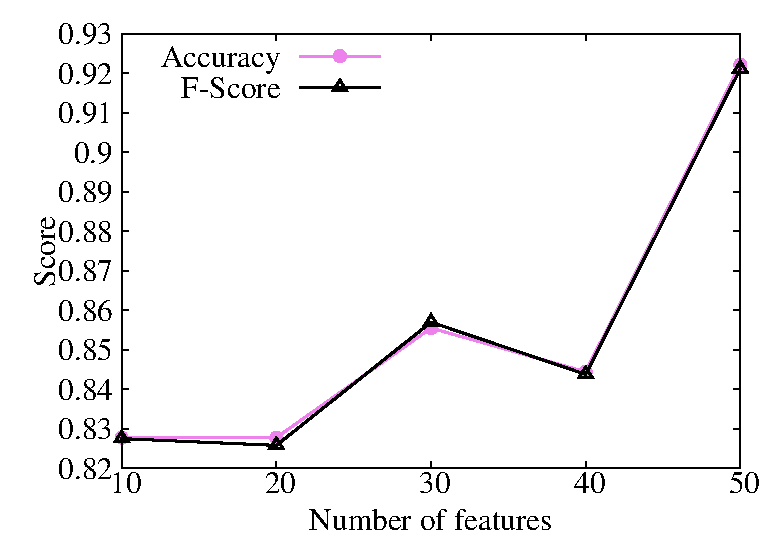
\includegraphics[scale=0.6] {Output/newTree/accuracy_fscore.eps}
 \caption { Decision Tree Classifier: Score vs Top K Features (Shuffled data set)} \label{acc_fscore}
 \end{center}
\end{figure}

As shown in Fig. \ref{acc_fscore}, the average accuracy and F-score achieved for different number of top K features (most frequent words) computed for shuffled data set is more or less same. It shows that both metrics (i) Accuracy and (ii) F-score works well for given data set.

\iffalse
\begin{figure}[h]
\begin{center}
\label{thr}
\subfigure[\label{cosine_1}]{
\epsfig{figure=Output/newKNN/accuracy.eps,width=2.5in,keepaspectratio}}
\subfigure[\label{cosine_2}]{
\epsfig{figure=Output/newKNN/fScore.eps,width=2.5in,keepaspectratio}}
\subfigure[\label{cosine_3}]{
\epsfig{figure=Output/newKNN/accuracy_fscore.eps,width=2.50in,keepaspectratio}}
\caption{ kNN classifier: Score vs Top K Features }
\end{center}
\end{figure}
\fi

\subsection{\underline{Evaluation of kNN}}
In this section, we evaluate K Neighbors classifier in terms of accuracy and F-score.
\begin{figure}[h]
\begin{center}
\label{thr}
\subfigure[\label{accuracy3}]{
\epsfig{figure=Output/newKNN/accuracy_unshuffled.eps,width=2.5in,keepaspectratio}}
\subfigure[\label{accuracy4}]{
\epsfig{figure=Output/newKNN/accuracy.eps,width=2.5in,keepaspectratio}}
\caption{ kNN Classifier: Accuracy vs (a. Unshuffled Data Matrix  b. Shuffled Data Matrix) }
\end{center}
\end{figure}

\begin{figure}[h]
\begin{center}
\label{thr}
\subfigure[\label{fscore3}]{
\epsfig{figure=Output/newKNN/fScore_unshuffled.eps,width=2.50in,keepaspectratio}}
\subfigure[\label{fscore4}]{
\epsfig{figure=Output/newKNN/fScore.eps,width=2.50in,keepaspectratio}}
\caption{ kNN Classifier: F-Score vs (a. Unshuffled Data Matrix  b. Shuffled Data Matrix) }
\end{center}
\end{figure}


As shown in Fig. \ref{accuracy3} and \ref{accuracy4}, the accuracy score achieved in shuffled training data set is higher than that of unshuffled training data set. As aforementioned, the reason is clustered labels in unshuffled data set (data matrix). Hence, the training is performed on a fixed set of clustered labels, whereas the testing is done against another chunk of dataset (which may have different set of clustered labels). 

Similar is the case with F-score values calculated over unshuffled data set and shuffled data set as shown in Fig. \ref{fscore3} and \ref{fscore4} respectively.


\begin{figure}[h]
\begin{center}
\subfigure[\label{knn_neigh}]{
\epsfig{figure=Output/knn_neigh_accuracy.eps,width=2.50in,keepaspectratio}}
\subfigure[\label{acc_fscore2}]{
\epsfig{figure=Output/newKNN/accuracy_fscore.eps,width=2.50in,keepaspectratio}}
 \caption {kNN Classifier: a. Avg. Accuracy vs Number of Neighbors  b. Score vs Top K Features (Shuffled data set)}
 \end{center}
\end{figure}

Fig \ref{knn_neigh} shows that the average accuracy achieved by kNN classifier is best when number of neighbors is low (such as $5$). However, when the number of neighbors increase, the accuracy dips. It is because with increase in number of neighbors, the far off neighbors with uncorrelated labels are also taken into consideration.

As shown in Fig. \ref{acc_fscore2}, the average accuracy score achieved is almost same as that computed using F-Score metric over shuffled data set for the kNN classifier. Hence, it shows that both metrics work well for given data set as well.

\begin{figure}[h]
\begin{center}
\label{thr}
\subfigure[\label{dt_knn1}]{
\epsfig{figure=Output/dt_knn1.eps,width=2.5in, keepaspectratio}}
\subfigure[\label{dt_knn2}]{
\epsfig{figure=Output/dt_knn2.eps,width=2.5in,keepaspectratio}}
\caption{ Decision Tree vs kNN classifier: (a. Accuracy b. F-Score) vs Top K features }
\end{center}
\end{figure}




\subsection{\underline{Decision Tree vs kNN }}
In this section, we present the evaluation results for the performance of Decision Tree and kNN classifiers for shuffled data set in terms of both metrics (i) Accuracy and (ii) F-Score



As shown in Fig. \ref{dt_knn1} and \ref{dt_knn2}, the decision tree classifier works better than kNN classifier. It is obvious because decision tree is robust, takes the weights of each feature in consideration to form a well-defined tree based on features list. Whereas, kNN is based on majority votes of k nearest neighbors. It is not able to capture the unequal weight of each feature.

\section{Conclusion}
From above analysis, it is evident that Decision Tree classifier works better than kNN classifier for a given data set. Also, it is clear that shuffled data set is preferred compared to unshuffled data set for training as it removes any clustered labels (polarized data sets). Moreover, both the metrics (i) Accuracy and (ii) F-Score works well for the given data set irrespective of number of features considered.

Lastly, the achieved score (using any metric) improves with higher number of features in both the classifiers which is quite intuitive.
\end{document}